\section{Introduction}
\label{ch:Introduction}

\begin{figure*}[hbt!]
    \centering
    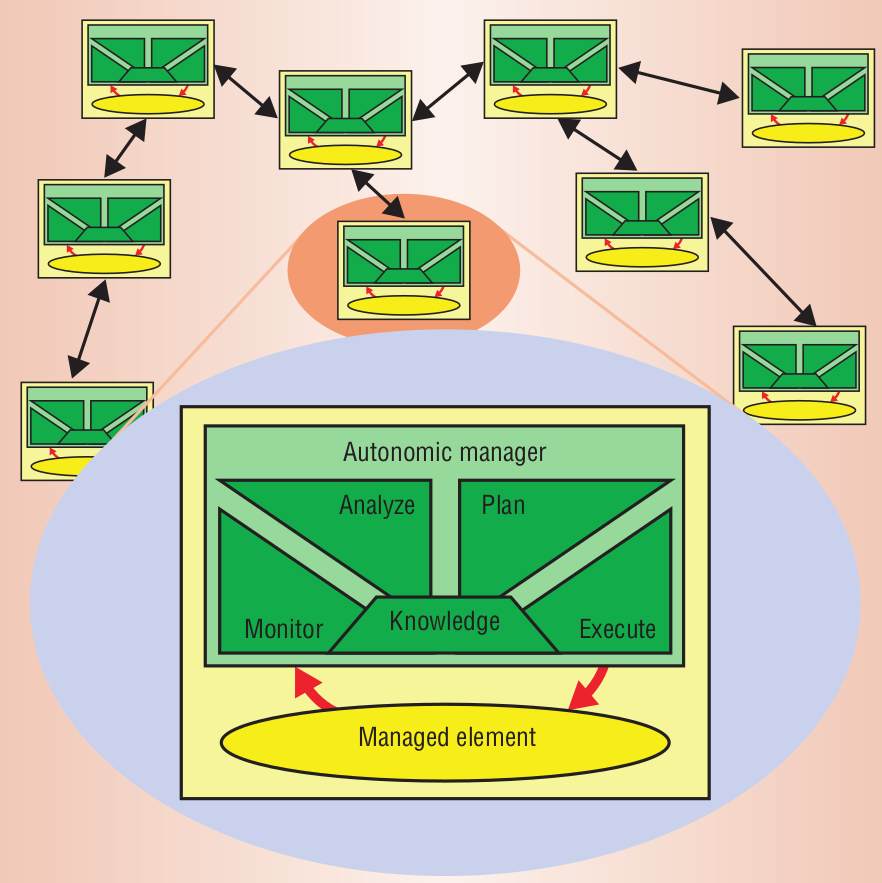
\includegraphics[width=0.6\textwidth]{images/MAPEK.png}
    \caption{The \acrshort{mapek} (Monitor-Analyze-Plan-Execute with Knowledge) feedback \cite*{VisionOfAutonomicComputing}}
    \label{fig:MAPEK}
\end{figure*}

The complexity of modern software systems is constantly growing.
Most of this growth in complexity stems from the
"need to integrate several heterogeneous environments into corporate-wide computing systems,
and to extend that beyond company boundaries into the Internet" \cite*{VisionOfAutonomicComputing}.
This has reached a state where the
"complexity appears to be approaching the limits of human capability" \cite*{VisionOfAutonomicComputing}.
In combination with the uncertainty about a software systems future operations and environment,
that the developers of such complex systems face, it becomes uneconomical to purely operate such a system by human operators.

\noindent From this the need for software systems which can autonomously manage themselves arises.
In order to achieve this task of autonomous self-management, the system has to be able to:
Detect faults and changes in its environment, analyze them, decide how to react to them and make changes to itself.

\noindent To model these abilities Kephart and Chess developed
the \acrfull{mapek} feedback loop \cite*{VisionOfAutonomicComputing} shown in Figure \ref{fig:MAPEK}.

\noindent First the system has to \textit{monitor} itself and its environment.
The data, gathered by the monitoring step, has to be \textit{analyzed} to detect changes and faults.
If the analyzing step detects, that an adaptation is necessary,
the system has to \textit{plan} how to perform the necessary changes.
After the changes have been planned, they need to be \textit{executed}.
All of this happens with \textit{knowledge} of the environment and the system.
This feedback loop can be used in a centralized way where one \textit{Autonomic manager} manages the complete system.
It can also be used in decentralized way with one \textit{Autonomic manager} per system component.
In this case the different \textit{Autonomic managers} can communicate with each other to exchange information about the system.

\noindent Software systems that can autonomously manage themselves are called self-adaptive
because of their ability to adapt themselves.

\noindent While \acrshort{sas} are better at handling more complex systems,
human operators are better at handling uncertainty.
This is because \acrshort{sas} can adapt the software that they are managing, but they can not adapt themselves,
because the adaptation rules and policies used by \acrshort{sas} are statically created at design time.
Over time this leads to an increasing divergence between the expected results of adaptations and the actual results,
when the environment changes in ways that were not predicted by developers during the design time of the system.

\noindent Optimizations are necessary to improve the performance and effectiveness of \acrshort{sas} in situations like these.
There are already many approaches on how to optimize \acrshort{sas}.
Some of them focus on updating adaptation rules and policies during the systems runtime.
Others dynamically change at which level of the system adaptations are performed.
Generally most optimizations target static components of \acrshort{sas}.
These components can be improved by making them more dynamic, 
which is often achieved by applying modern learning methods.

\noindent While there are already many \acrshort{oa} for \acrshort{sas},
there is no classification for them.
Because of this, the existing \acrshort{oa} can not be easily compared
and it is difficult to identify areas which require further research.
This paper aims to provide such a classification for \acrshort{oa} for \acrshort{sas}.
The proposed classification will then be used to compare existing \acrshort{oa}.

\noindent Chapter \ref{ch:Foundations} provides some foundational knowledge about \acrshort{sas}.
To derive a classification for \acrshort{oa} for \acrshort{sas},
chapter \ref{ch:SASClassification} will first explain how \acrshort{sas} are classified
using three different approaches.
Based on these approaches, a classification for \acrshort{oa} for \acrshort{sas} will be derived
and proposed in chapter \ref{ch:Proposal}.
In chapter \ref{ch:Existing} the proposed classification will be applied to some existing \acrshort{oa}.
Lastly, chapter \ref{ch:Conclusion} will finish with a conclusion and recommendations for future research directions.
